\documentclass[Arkitektur/System_main.tex]{subfiles}

\begin{document}
I det følgende gives en beskrivelse af arkitekturen for Beerpong Table. Formålet med arkitekturen er at beskrive, hvordan systemet er opbygget, og hvordan dets forskellige elementer fungerer. For at give en grundig beskrivelse af systemets funktionalitet og sammensætning, er arkitekturen opdelt i sekvensdiagrammer og henholdsvis system-, hardware- og softwarearkitektur.

\section{Systemarkitektur} \label{sec:systemarkitektur}

 Indledningsvis er kombinationen af hardware og software vist i et deployment view i figur \ref{fig:systemarkitektur}. Det viser hvordan softwareapplikationer er allokeret på de tre dele af systemet, som indeholder CPU'er. Det er blokkene Player side, RPi og Ball dispenser, som er beskrevet nærmere i den tilhørende blokbeskrivelse.


\begin{figure}[H]
    \centering
    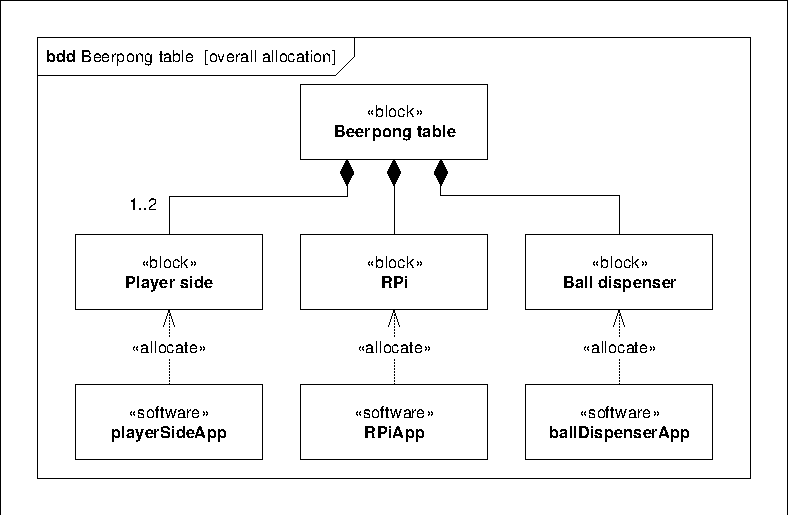
\includegraphics[width=1\textwidth,trim={0.24in 0.24in 0.24in 0.24in},clip, page=1]{Arkitektur/graphics/BDD_og_IBD.pdf}
    \caption{Overordnet blok definitionsdiagram for systemet med software allokeringer. Indeholder kun blokke med CPU}
    \label{fig:systemarkitektur}
\end{figure}

\subsection{Blokbeskrivelse} \label{sec:system_block_description}

\begin{table}[H]
\centering
\begin{tabular}{|L{0.2\columnwidth}|L{0.7\columnwidth}|}
\hline
\textbf{Blok} & \textbf{Beskrivelse} \\ \hline
Player side & Skal sørge for at håndtere alt med hensyn til kopperne på den ene ende af bordet. Den skal derfor registrere når en kop fjernes. Og den skal også styre lyset under hver kop. (Evt. skal den også registrere når en bold rammer i en kop) \newline CPU'en i Player side er en PSoC. \\ \hline
RPi & Har til ansvar at styre spillets gang. Den får informationer om de forskellige sensorer fra de andre CPU'er i systemet. Derudover får den også information fra en hjemmeside som den hoster. Den skal på baggrund af disse informationer styre de forskellige aktuatorer vha. de andre CPU'er. Den skal også styre hvad der vises på en skærm. \newline CPU'en i RPi er en Raspberry pi zero W  \\ \hline
Ball dispenser & Skal modtage mønter fra brugeren og fortælle RPi om dette. Den skal levere en bordtennisbold når den får besked om det fra RPi. Når den er løbet tør for bolde, skal den informere RPi om dette. Den skal også have lys til at informere bruger og servicemedarbejder om status på bolddispenseren. \newline CPU'en i Ball dispenser er en PSoC.  \\ \hline
\end{tabular}
\end{table}

\end{document}